\documentclass{article}
\usepackage{graphicx} % Required for inserting images
\usepackage[french]{babel}
\usepackage{multirow}
\usepackage[utf8]{inputenc}
\usepackage[a4paper,margin=0.5in]{geometry}
\usepackage[T1]{fontenc}
\usepackage{amsmath}
\usepackage{amsthm}
\usepackage{amsfonts}
\usepackage{amsmath}
\usepackage{amssymb}
\usepackage{adjustbox}
\usepackage{array}
\usepackage{algorithm}
\usepackage{algorithmic}
\usepackage{siunitx} % Pour la notation scientifique
\usepackage{graphicx}
\usepackage{subcaption} % Pour les sous-figures
\usepackage{booktabs} % Pour de meilleurs tableaux
\usepackage{subcaption}  % Nécessaire pour les sous-figures



\begin{document}

\begin{titlepage}
\begin{center}
    
\includegraphics[width=0.3\linewidth]{Logo-toulouse-inp-N7.png}
\end{center}
    \centering
    \vspace*{3in} % Ajuste la hauteur pour centrer verticalement
    \Huge \textbf{Rapport VDA} \\[1cm] % Titre
    \Large {Par Axel OLOUGOUNA et Ayoub CHOUKRI} \\ % Auteu
    \Large \date{March 2025} % Date
    \vfill
\end{titlepage}

\newpage

\tableofcontents

\newpage


\section{Introduction} 

Ce TP vise à estimer la bathymétrie \( b(x) \) d'une rivière à partir de mesures de surface \( H^{obs}(x) \) en utilisant un modèle d'écoulement simplifié. Nous étudierons d'abord le modèle direct pour comprendre l’influence de \( b(x) \) sur la surface de l’eau, puis résoudrons un problème inverse d’optimisation pour retrouver \( b(x) \) à partir des observations. L’analyse portera sur la sensibilité du modèle et l’impact des paramètres de régularisation.

\section{Étude du modèle}

\subsection{Modèle Direct}
Le modèle qui lie la bathymétrie \( b \) à la hauteur de l'eau \( H \) est le suivant :

\[
-\Lambda_{\text{ref}}(b)\partial^{2}_{xx}H(x) + \partial_{x}H(x) + \frac{\partial_{x}w(x)}{w(x)}H(x) = \partial_{x}b(x) + \frac{\partial_{x}w(x)}{w(x)}b(x)
\quad \text{(1)}
\]

Les conditions aux limites sont de type Dirichlet non homogènes. La diffusivité effective est donnée par une solution de référence \( H_{\text{ref}}(x) \) :

\[
\Lambda_{\text{ref}}(b) = \frac{3}{10}\frac{(H_{\text{ref}}(x) - b(x))}{|\partial_{x}H_{\text{ref}}(x)|}
\]


\subsection{Formulation faible}
Dans cette partie, on va essayer de retrouver la formulation faible de notre EDP: \newline 

Partons de l'équation forte du modèle (1). Pour obtenir sa formulation variationnelle :  

1. \textbf{Multiplication par une fonction test} :  
Soit \( v \in H^1_0(\Omega) \) une fonction test s'annulant aux bords. Multiplions les deux membres de (1) par \( v \) :  
\[
\int_\Omega \left(-\Lambda_{\text{ref}}(b)\partial_{xx}^2H + \partial_xH + \frac{\partial_xw}{w}H\right)v \, dx = \int_\Omega \left(\partial_xb + \frac{\partial_xw}{w}b\right)v \, dx
\]

2. \textbf{Application de la formule de Green} :  
Appliquée au terme diffusif d'ordre 2, avec \( \mathbf{n} \) le vecteur normal sortant unitaire :  
\[
-\int_\Omega \Lambda_{\text{ref}}(b)\partial_{xx}^2H \, v \, dx = \int_\Omega \partial_x(\Lambda_{\text{ref}}(b)\partial_xH) \, v \, dx - \int_{\partial\Omega} \Lambda_{\text{ref}}(b)(\partial_xH \cdot \mathbf{n}) \, v \, d\Gamma
\]  
Le terme de bord s'annule car \( v \in H_0^1(\Omega) \).  

3. \textbf{Formulation faible finale} :  
En regroupant les termes, on obtient la forme bilinéaire \( a(b; H, v) \) et la forme linéaire \( l(b; v) \) :  
\[
\boxed{
\begin{aligned}
a(b; H, v) &= \int_\Omega \partial_x(\Lambda_{\text{ref}}(b) \partial_xH) \, v \, dx + \int_\Omega \partial_xH \, v \, dx + \int_\Omega \frac{\partial_xw}{w} H \, v \, dx, \\
l(b; v) &= \int_\Omega \left(\partial_xb + \frac{\partial_xw}{w}b\right)v \, dx.
\end{aligned}
}
\]  
La formulation faible s'écrit alors :  
\[
a(b; H, v) = l(b; v) \quad \forall v \in H^1_0(\Omega). \tag{3}
\]  
Cette forme est adaptée à une discrétisation par éléments finis.  

\subsection{Modèle adjoint}



Par définition, le modèle adjoint en formulation faible s'écrit :  
\[
a^*(b; P, z) = \partial_H a(b; H^b; P) \cdot z \quad \forall z \in V
\]  

Comme le modèle est linéaire en \( H \), la dérivée partielle \( \partial_H a(b; H^b; P) \) coïncide avec la forme bilinéaire évaluée en \( P \). On obtient directement :  
\[
a^*(b; P, z) = a(b; z, P) 
\]  

Explicitement, pour tout \( z \in V = H^1_0(\Omega) \) :  
\[
a^*(b; P, z) = \int_\Omega \partial_x(\Lambda_{\text{ref}}(b) P) \, \partial_x z \, dx - \int_\Omega \partial_x P \, z \, dx + \int_\Omega \frac{\partial_x w}{w} P z \, dx \tag{14}
\]  

L'équation adjointe devient alors :  
\[
a^*(b; P, z) = \int_\Omega J'_{\text{obs}}(H^b) \, z \, dx \quad \forall z \in V. \tag{13}
\]  


\subsection{Passage à la forme classique}  
En exploitant l'intégration par parties et les conditions \( P|_{\partial\Omega} = 0 \), le terme diffusif devient :  
\begin{equation}
\int_\Omega \partial_x\left(\Lambda_{\text{ref}}(b) P\right) \partial_x z \, dx = -\int_\Omega \partial_{xx}^2\left(\Lambda_{\text{ref}}(b) P\right) z \, dx. \tag{15}
\end{equation}  
L'équation (13) se réécrit alors :  
\begin{equation}
\int_\Omega \left(-\partial_{xx}^2\left(\Lambda_{\text{ref}}(b) P\right) - \partial_x P + \frac{\partial_x w}{w} P \right) z \, dx = \int_\Omega J'_{\text{obs}}(H^b) z \, dx. \tag{16}
\end{equation}  

Par le théorème de représentation de Riesz-Fréchet, on identifie la forme linéaire à une fonction dans \( L^2(\Omega) \). Ceci conduit à la forme forte du modèle adjoint :  
\begin{equation}
-\partial_{xx}^2\left(\Lambda_{\text{ref}}(b) P\right) - \partial_x P + \frac{\partial_x w}{w} P = J'_{\text{obs}}(H^b) \quad \text{dans } V'. \tag{17}
\end{equation}


\section{Expression du gradient}

\subsection{Fonction objectif}
La fonction coût globale s'écrit comme la somme d'un terme d'observation et d'un terme de régularisation :
\begin{equation}
J(b; H) = J_{\text{obs}}(H) + \alpha_{\text{reg}} J_{\text{reg}}(b), \tag{19}
\end{equation}
où \( \alpha_{\text{reg}} > 0 \) est un paramètre de pénalisation. Pour \( j(b) = J(b; H^b) \), la différentielle de \( j \) s'exprime par :  
\begin{equation}
j'(b) \cdot \delta b = \left( \alpha_{\text{reg}} J'_{\text{reg}}(b) - \left[ \frac{\partial a}{\partial b}(b; H^b, P^b) - \frac{\partial l}{\partial b}(b; P^b) \right] \right) \cdot \delta b, \quad \forall \delta b. \tag{20}
\end{equation}

\subsection{Forme explicite du gradient}  
En développant les termes de (20), on obtient :  
\[                                                                                                                                                                                                                                       
j'(b) \cdot \delta b = \alpha_{\text{reg}} J'_{\text{reg}}(b) \cdot \delta b 
- \int_\Omega \partial_x\left(\Lambda'_{\text{ref}}(b) P^b(x)\right) \partial_x H^b(x) \, dx 
+ \int_\Omega \left( \partial_x(\delta b)(x) + \frac{\partial_x w(x)}{w(x)} \delta b(x) \right) P^b(x) \, dx, \tag{21}
\]  
avec \( \Lambda'_{\text{ref}}(b) = -\frac{3}{10} \frac{\delta b(x)}{|\partial_x H_{\text{ref}}(x)|} \).

\subsection{Exemples de termes de régularisation}  
\begin{itemize}
\item \textbf{Régularisation de la dérivée} :  
\( J_{\text{reg}}(b) = \|\partial_x b - \partial_x H_{\text{ref}}\|_{L^2}^2 \), donnant :  
\[
J'_{\text{reg}}(b) \cdot \delta b = 2 \int_\Omega (\partial_x b - \partial_x H_{\text{ref}}) \partial_x (\delta b) \, dx.
\]

\item \textbf{Régularisation de la bathymétrie} :  
\( J_{\text{reg}}(b) = \|b - b_{\text{prior}}\|_{L^2}^2 \), donnant :  
\[
J'_{\text{reg}}(b) \cdot \delta b = 2 \int_\Omega (b - b_{\text{prior}}) \delta b \, dx.
\]
\end{itemize}

\subsection{Test du gradient}

Afin de s'assurer de la validité de notre modèle adjoint, on compare le gradient obtenu à travers le modèle adjoint avec différents types de différences finies pour approximer le gradient, d'ordre 1 (à gauche ou à droite) et d'ordre 2 (centrée).

Le test repose sur le développement de Taylor :
\[
j(b_0 + \varepsilon \delta b) = j(b_0) + \varepsilon \frac{\partial j}{\partial b}(b_0) \cdot \delta b + o(\varepsilon \| \delta b \|).
\]

On en déduit les formules des différences finies suivantes :

\begin{itemize}
    \item Ordre 1 (différence avant ou arrière) :
    \[
    I_\varepsilon = \frac{j(b_0 + \varepsilon \delta b) - j(b_0)}{\varepsilon \cdot \frac{\partial j}{\partial b}(b_0) \cdot \delta b}
    \]
    
    \item Ordre 2 (différence centrée) :
    \[
    I_\varepsilon = \frac{j(b_0 + \varepsilon \delta b) - j(b_0 - \varepsilon \delta b)}{2 \varepsilon \cdot \frac{\partial j}{\partial b}(b_0) \cdot \delta b}
    \]
\end{itemize}

Pour vérifier si le gradient est bien approché, on vérifie que :
\[
\lim_{\varepsilon \to 0} I_\varepsilon = 1
\]

Pour cela, on trace \( \left| 1 - I_{\varepsilon_n} \right| \) en fonction de \( \varepsilon_n \), en échelle logarithmique :

\begin{figure}[H]
    \centering
    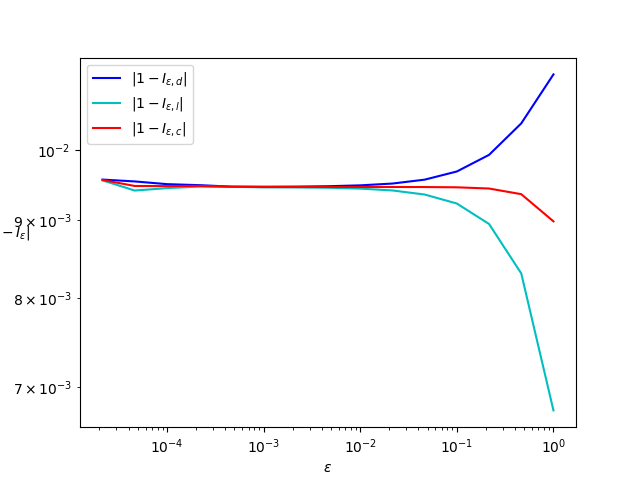
\includegraphics[width=0.8\linewidth]{Images_Axel/grad2.png}
    \caption{Évolution de \( | 1 - I_\varepsilon | \) en fonction de \( \varepsilon \) }
    \label{fig:grad-test}
\end{figure}

On constate que \( | 1 - I_\varepsilon | \) converge vers $0$ quand lorsque $\epsilon$  tombe vers $0$, confirmant la validité du gradient calculé via le modèle adjoint.


\section{Non-unicité du contrôle \( b(x) \)}
\label{subsec:non_unicite}

D'après l'analyse présentée lors des séances de TP (cf. document complémentaire), il peut exister plusieurs solutions \( b(x) \) pour une même hauteur d'eau \( H(x) \) observée. Ceci a été démontrée via l'équation suivante:

\begin{equation}
b_2(x) = b_1(x) + (b_2 - b_1)(x_0) \left(\frac{|H^{\prime}(x)|^{\frac{3}{10}}}{w(x)}\right)
\label{eq:non_unicite}
\end{equation}

\subsection{Rôle de la régularisation}
L'équation du modèle direct étant linéaire en la hauteur d'eau \( H \), et compte tenu de la fonction coût qui s'écrit :

\begin{equation}
J(b) = \frac{1}{2}\|H(b) - H_{\text{obs}}\|^2 + \alpha_{\text{reg}} R(b)
\label{eq:loss}
\end{equation}

où \( R(b) \) représente le terme de régularisation, on distingue trois cas principaux :

\subsubsection{Régularisation \( L^2 \) de la bathymétrie}
\begin{equation}
R(b) = \frac{1}{2}\|b - b_{\text{background}}\|^2
\end{equation}

\textbf{Avantages} :
\begin{itemize}
\item Lorsque \( \alpha_{\text{reg}} \) est suffisamment grand, le problème devient un \textbf{problème linéaire-quadratique strictement convexe}
\item La fonction coût \( J(b) \) admet alors un unique minimum global \( b^* \)
\item La solution numérique converge systématiquement vers cette solution unique
\end{itemize}

\textbf{Inconvénients}
\begin{itemize}

        \item Forte dépendance à $b_b$ : Si $b_b$ est mal choisi, la régularisation peut mener à une mauvaise solution.
        \item Il ne contrôle ni la pente ni la régularité de $b$, contrairement aux régularisations de dérivées.
\end{itemize}

\subsubsection{Régularisation de la dérivée première}
\begin{equation}
R(b) = \frac{1}{2}\|\partial_x b - \text{Mean}(H^{\prime})\|^2
\end{equation}

\textbf{Avantages}
\begin{itemize}
\item On veille à obtenir une pente proche de \( \text{Mean}(H') \), ce qui est physiquement justifié.

\end{itemize}

\textbf{Inconvénients}
\begin{itemize}
    \item Le terme $\text{Mean}(H')$ peut être difficile à estimer de manière fiable.
\item Unicité non garantie (problème potentiellement non convexe)
\end{itemize}

\subsubsection{Régularisation de la dérivée seconde} 
\begin{equation}
R(b) = \frac{1}{2}\|\partial_{xx}^2 b\|^2
\end{equation}

\textbf{Avantages}
\begin{itemize}
\item Produit des solutions assez régulières


\end{itemize}

\textbf{Inconvénients}
\begin{itemize}
    \item Peut lisser à l’excès et effacer des structures physiques significatives (hautes fréquences de $b(x)$).
    \item Peut introduire un biais en faveur de profils trop homogènes.

    \item En présence de multiples minima locaux, l'algorithme peut converger vers une solution sous-optimale.
\end{itemize}


\paragraph{Sélection de la solution numérique} 
Lorsque plusieurs solutions $b(x)$ sont mathématiquement possibles pour un même $H(x)$ observé (cf. Éq.~\ref{eq:non_unicite}), la solution obtenue numériquement est déterminée par le terme de régularisation dominant dans la fonction coût $J(b)$ (Éq.~\ref{eq:loss}) : avec une régularisation $L^2$ forte ($\alpha_{\text{reg}} \gg 1$), on obtient systématiquement la solution unique $b^*$ proche de $b_{\text{background}}$ (problème LQ strictement convexe).




\section{Analyse du modèle direct}

On utilise les paramètres ci-après pour obtenir des résultats numériques.

\begin{table}[H]
\centering
\begin{tabular}{|l|c|l|}
\hline
\textbf{Paramètre} & \textbf{Valeur} & \textbf{Description} \\
\hline
\( L \) & \( 100 \times 10^3 \, \text{m} \) & Longueur du domaine \\
\( n_{\text{pts}} \) & 1001 & Nombre de points de grille \\
\( \text{slope} \) & \( 1 \times 10^{-3} \) & Pente du fond \\
\( h_{\text{ref}} \) & 10.0 m & Profondeur de l'eau (conditions de Dirichlet) \\
\( n\_{\text{wave\_bathy}} \) & 5 & Nombre d'ondes dans la bathymétrie \\
\( \text{amp}\_{\text{wave\_bathy}} \) & \( \frac{h_{\text{ref}}}{5} = 2.0 \, \text{m} \) & Amplitude des ondes de bathymétrie \\
\( \omega \) & \( \frac{2\pi}{L} \) & Fréquence spatiale des ondes \\
\hline
\end{tabular}
\caption{Paramètres du modèle}
\label{tab:parametres}
\end{table}


Le modèle direct relie la bathymétrie $b(x)$ à la hauteur d'eau $H(x)$ par l'équation aux dérivées partielles (1), et sa solution est notée $H^b = \mathcal{M}(b)$. Nous analysons ici la sensibilité de la « signature de surface » $H(x)$.

\subsection{Comportement de filtrage du modèle}

La structure du modèle révèle que $H$ est une solution lissée, notamment à travers le terme diffusif :
\[
-\Lambda_{\text{ref}}(b)\,\partial_{xx}^2 H.
\]
Ce terme agit comme un \textbf{filtre passe‑bas} spatial, atténuant les hautes fréquences de la bathymétrie et laissant passer les basses fréquences.

\begin{figure}[H]
    \centering
    \begin{minipage}[b]{0.45\linewidth}
        \centering
        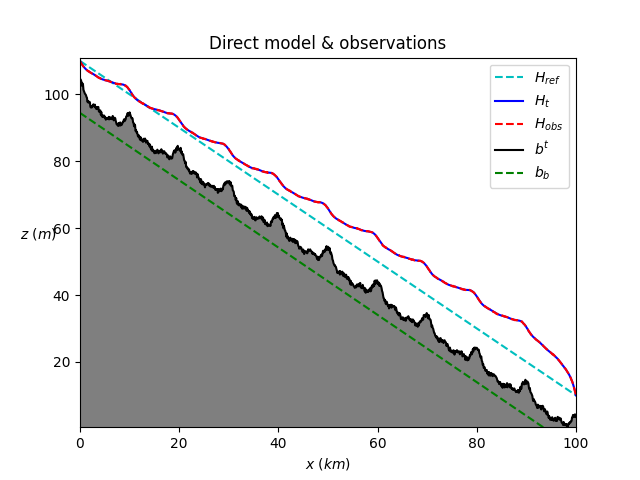
\includegraphics[width=\linewidth]{Images_Axel/n_wave_bathy_5.png}
        \caption{Bathymétrie avec n\_wave\_bathy = 5 (basse fréquence) et amplitude = 2 m}
        \label{fig:bathy_low}
    \end{minipage}
    \hfill
    \begin{minipage}[b]{0.45\linewidth}
        \centering
        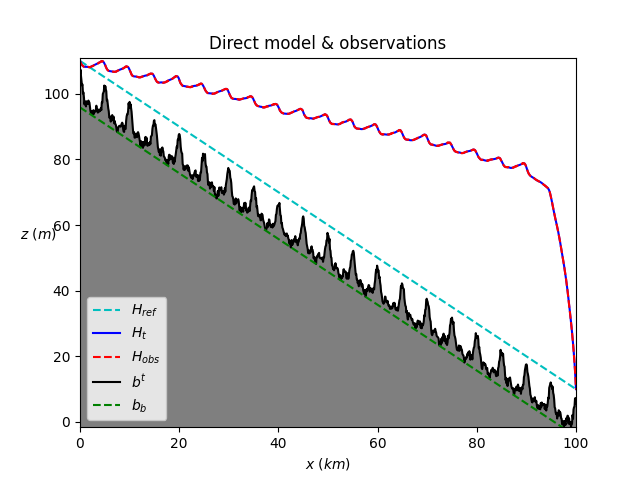
\includegraphics[width=\linewidth]{Images_Axel/n_20_amp_3.png}
        \caption{Bathymétrie avec n\_wave\_bathy = 20 (haute fréquence) et amplitude = 3.33 m}
        \label{fig:bathy_high}
    \end{minipage}
    \caption*{\small Comparaison entre deux bathymétries de fréquences différentes et d'amplitude pour illustrer l’effet de lissage de $H(x)$.}
    \label{fig:bathy_all}
\end{figure}

Le modèle agit comme un \textbf{filtre passe-bas}, rendant $H(x)$ surtout sensible aux variations lentes de $b(x)$. Les fortes pentes et faibles profondeurs ($H-b$ petit) produisent les signatures les plus marquées.

Les propriétés les plus sensibles à la signature de surface $H(x)$ sont donc :
\begin{itemize}
    \item \textbf{Profondeur} $H-b$ : influence la diffusivité $\Lambda_{\text{ref}}(b)$ 
    \item \textbf{Basses fréquences} : mieux résolues que les hautes fréquences (effet de lissage)
\end{itemize}

\subsection{Conséquences pour le problème inverse}

Ce filtrage implique que :
\begin{itemize}
    \item Les hautes fréquences de $b(x)$ sont mal transmises dans $H(x)$ et donc difficiles à inverser.
    \item Une \textbf{régularisation} est indispensable pour compenser cette perte d’information.
\end{itemize}


\section{Influence de la régularisation et/ou de $b_{1st}$ et $b_b$}


Dans cette partie on a décidé d'essayer différents choix de types de régularisation tout en modifient les valeurs initiales de la bathymétrie et / ou la bathymétrie background.

Pour la bathymétrie initiale, on a généralement utilisé : 


$$b_{\text{first}} = H_{\text{obs}} - c \cdot \text{prior\_depth} $$




\subsection{Sans aucune régularisation}


Dans cette section, on a décidé d'effectuer une résolution sans imposer aucune régularisation. 





\begin{figure}[H]
    \centering
    % Première ligne : Costs et Gradient
    \begin{minipage}[b]{0.45\linewidth}
        \centering
        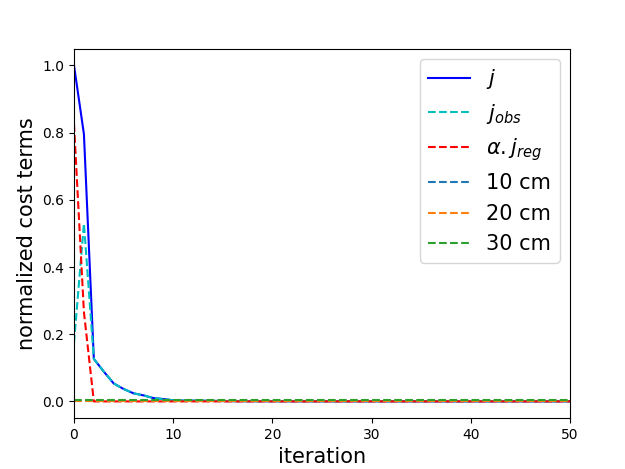
\includegraphics[width=\linewidth]{Images_Ayoub/No_Regularisation/Costs.png}
        \caption{Évolution des coûts sans régularisation.}
        \label{fig:costs}
    \end{minipage}
    \hfill
    \begin{minipage}[b]{0.45\linewidth}
        \centering
        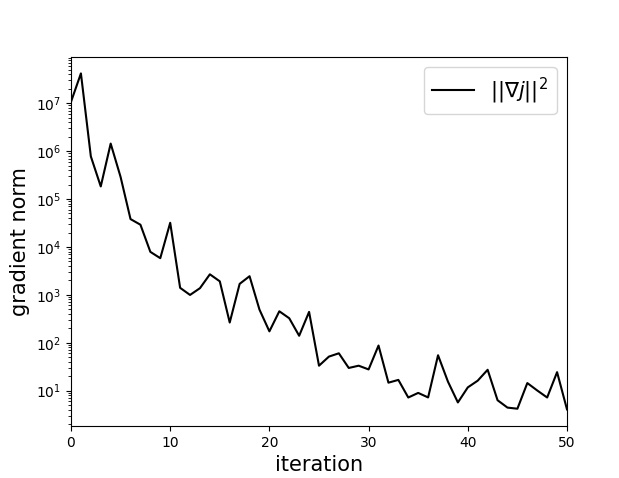
\includegraphics[width=\linewidth]{Images_Ayoub/No_Regularisation/Gradient.png}
        \caption{Champ de gradient sans régularisation.}
        \label{fig:gradient}
    \end{minipage}

    %\vspace{0.2cm}

    % Deuxième ligne : H et b
    \begin{minipage}[b]{0.45\linewidth}
        \centering
        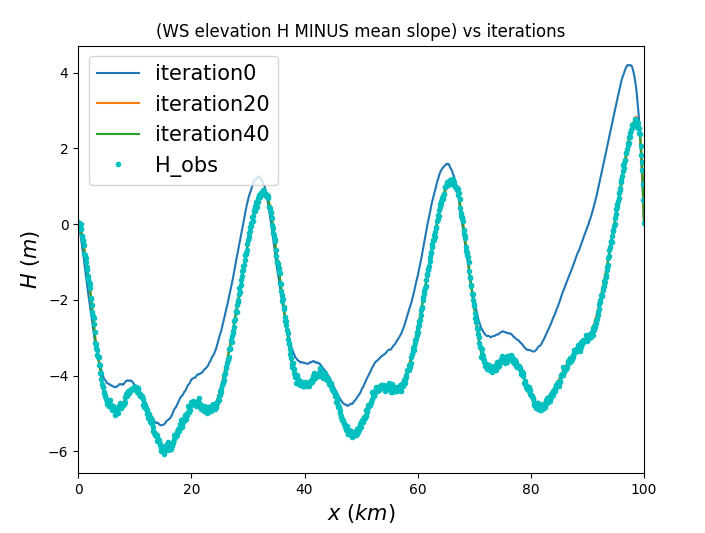
\includegraphics[width=\linewidth]{Images_Ayoub/No_Regularisation/H_Comparaison.png}
        \caption{Comparaison de $H$ sans régularisation.}
        \label{fig:h-comparaison}
    \end{minipage}
    \hfill
    \begin{minipage}[b]{0.45\linewidth}
        \centering
        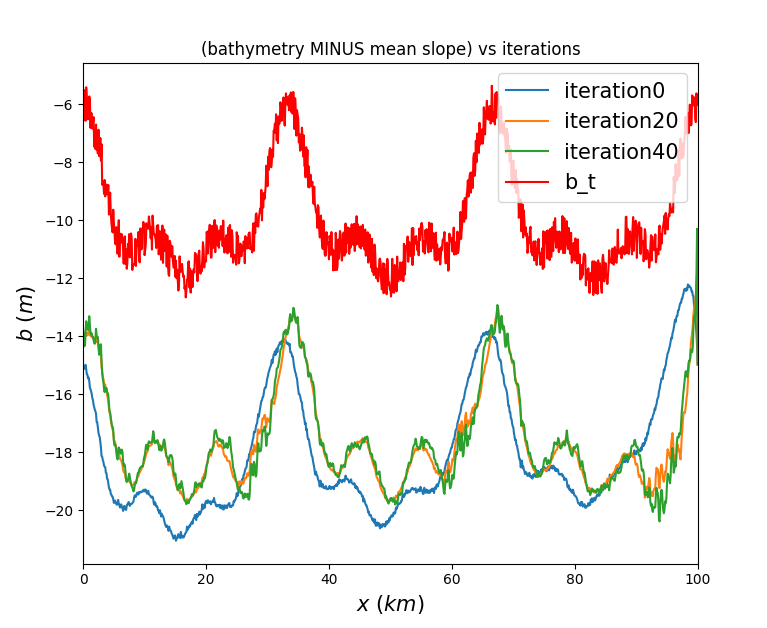
\includegraphics[width=\linewidth]{Images_Ayoub/No_Regularisation/b_Comparaison.png}
        \caption{Comparaison de $b$ sans régularisation.}
        \label{fig:b-comparaison}
    \end{minipage}

    %\vspace{0.5cm}

    % Troisième ligne : View
    \begin{minipage}[b]{0.55\linewidth}
        \centering
        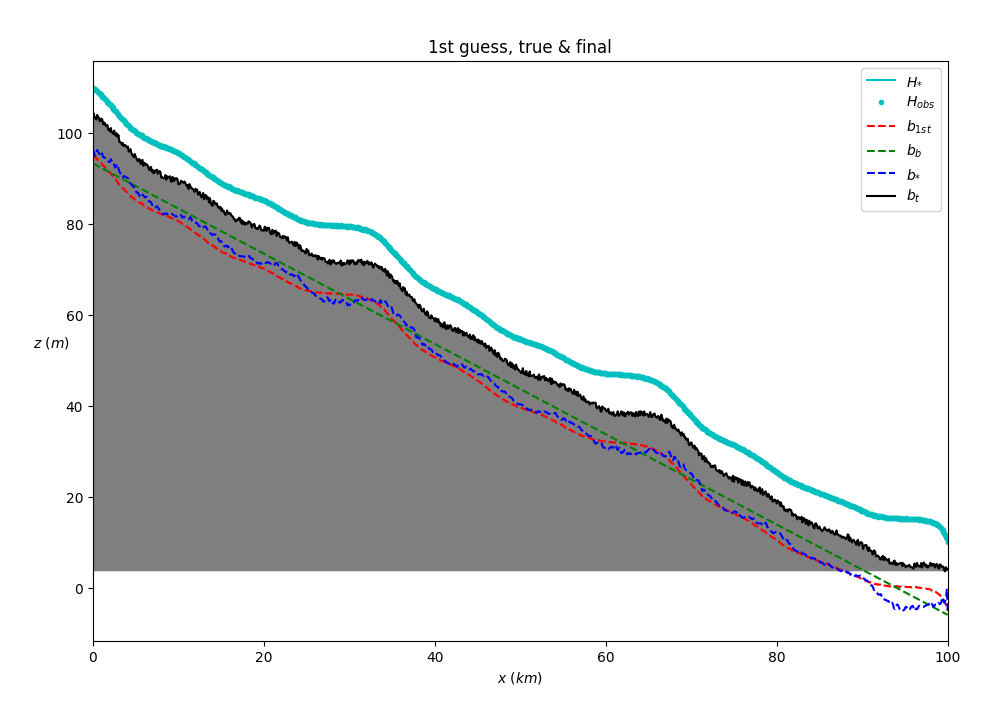
\includegraphics[width=\linewidth]{Images_Ayoub/No_Regularisation/View.png}
        \caption{Vue du champ simulé sans régularisation.}
        \label{fig:view}
    \end{minipage}
\end{figure}


\paragraph{Analyse des résultats}
Les fonctions de coût décroissent assez bien ; le fait que la norme du gradient ne soit pas strictement nulle en fin d’optimisation peut surprendre, mais cela s’explique par les contraintes imposées lors de la minimisation. On peut résumer ces observations comme suit :

\begin{itemize}
  \item Les coûts diminuent rapidement et se stabilisent vers une valeur minimale, attestant d’une convergence satisfaisante.
  \item La norme du gradient \(\|\nabla J\|\) ne s’annule pas complètement à la fin de l’optimisation, en raison des contraintes d'inégalité  imposée à la bathymétrie $b$.
  \item La hauteur de l'eau \(H\) est très bien approchée : la solution finale coïncide quasiment avec les observations.
  \item En revanche, l’estimation du fond \(b\) s’écarte significativement de la valeur a priori.
  \item En l’absence de régularisation, rien ne contraint \(b\) à rester proche de sa valeur background, d’où ces dérives.
  \item Il serait pertinent d’introduire un terme de régularisation, ou une pénalité spatiale pour canaliser les variations non‑physiques du fond lors de l’inversion.
\end{itemize}


\subsection{Avec une régularisation type Background}
\subsubsection{Avec $\alpha_{reg}$ constant}
Après avoir comparé les ordres de grandeur initiaux, à savoir \(J_{\rm obs}(0)=1.6382\times10^5\) et \(J_{\rm reg}(0)=7.9424\times10^5\), il est apparu nécessaire de retenir \(\alpha=\tfrac{1}{8}\) afin d’équilibrer les deux contributions de la fonction de coût.


\begin{figure}[H]
    \centering
    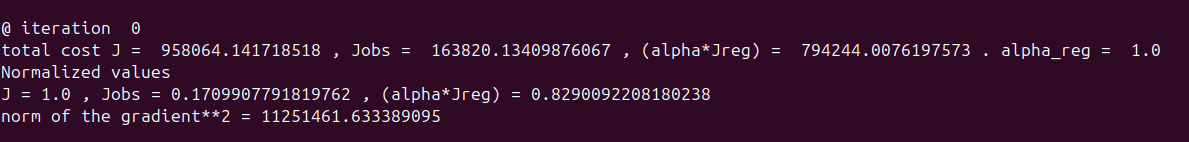
\includegraphics[width=0.8\linewidth]{Images_Ayoub/With_Regularisation/Alpha_Const/Pasted image.png}
    \caption{Valeurs des Los à l'itération 0}
    \label{fig:enter-label}
\end{figure}

\begin{figure}[H]
    \centering
    % Première ligne : Costs et Gradient
    \begin{minipage}[b]{0.45\linewidth}
        \centering
        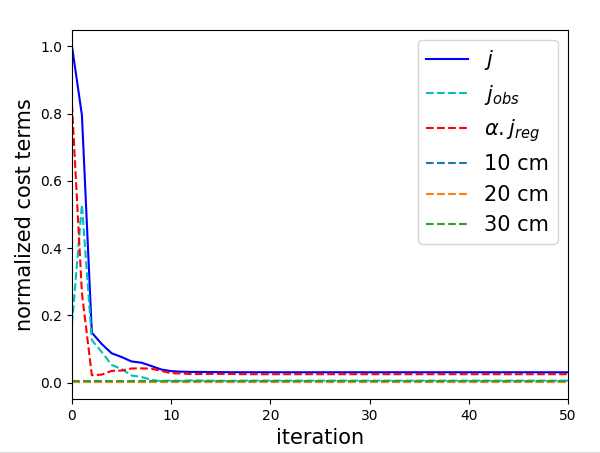
\includegraphics[width=\linewidth]{Images_Ayoub/With_Regularisation/Alpha_Const/Graphs/Costs.png}
        \caption{Évolution des coûts avec \(\alpha=\tfrac18\).}
        \label{fig:wr-costs}
    \end{minipage}
    \hfill
    \begin{minipage}[b]{0.45\linewidth}
        \centering
        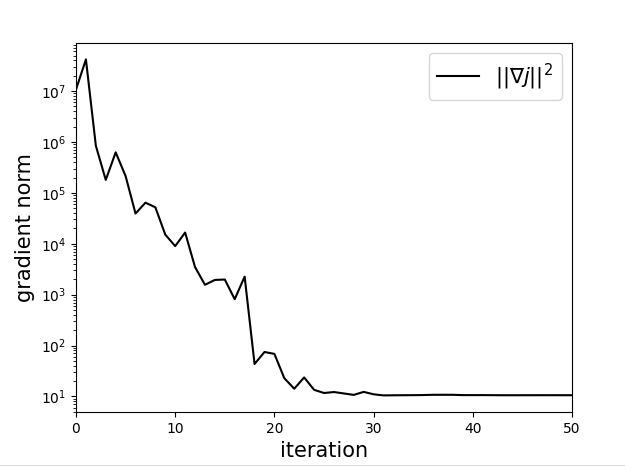
\includegraphics[width=\linewidth]{Images_Ayoub/With_Regularisation/Alpha_Const/Graphs/Gradient.png}
        \caption{Norme du gradient avec \(\alpha=\tfrac18\).}
        \label{fig:wr-gradient}
    \end{minipage}

    %\vspace{0.5cm}

    % Deuxième ligne : RMSE et b_Comparaison
    \begin{minipage}[b]{0.45\linewidth}
        \centering
        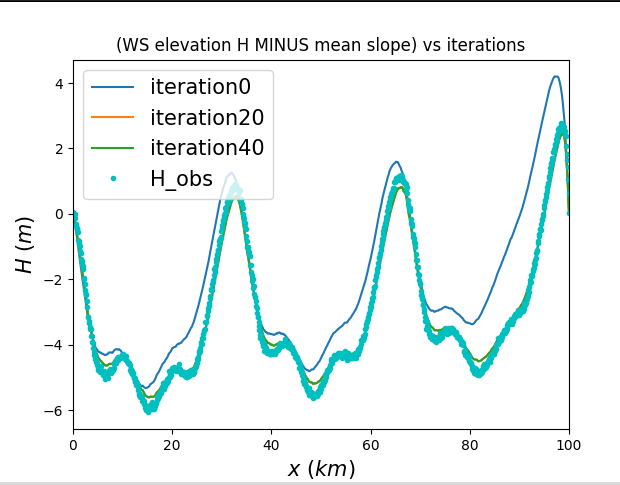
\includegraphics[width=\linewidth]{Images_Ayoub/With_Regularisation/Alpha_Const/Graphs/H_Comparaison.png}
        \caption{Comparaison de $H$}
        \label{fig:wr-rmse}
    \end{minipage}
    \hfill
    \begin{minipage}[b]{0.45\linewidth}
        \centering
        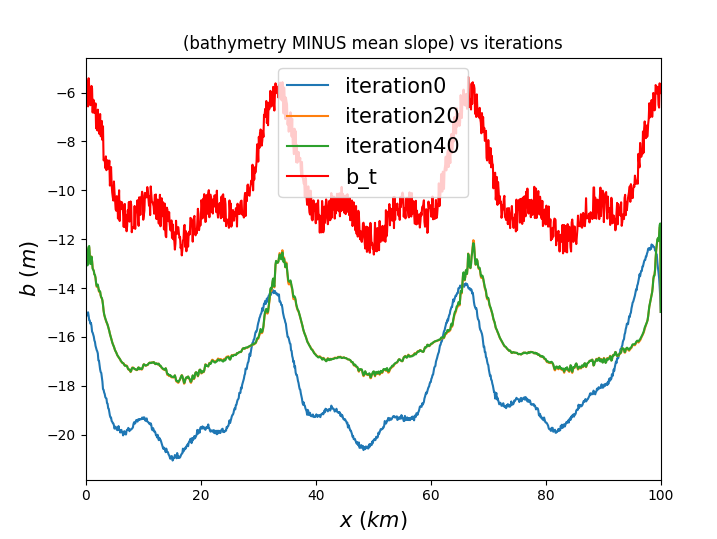
\includegraphics[width=\linewidth]{Images_Ayoub/With_Regularisation/Alpha_Const/Graphs/b_Comparaison.png}
        \caption{Comparaison du fond \(b\) avec la référence.}
        \label{fig:wr-b-comparaison}
    \end{minipage}

    %\vspace{0.5cm}

    % Troisième ligne : View
    \begin{minipage}[b]{0.6\linewidth}
        \centering
        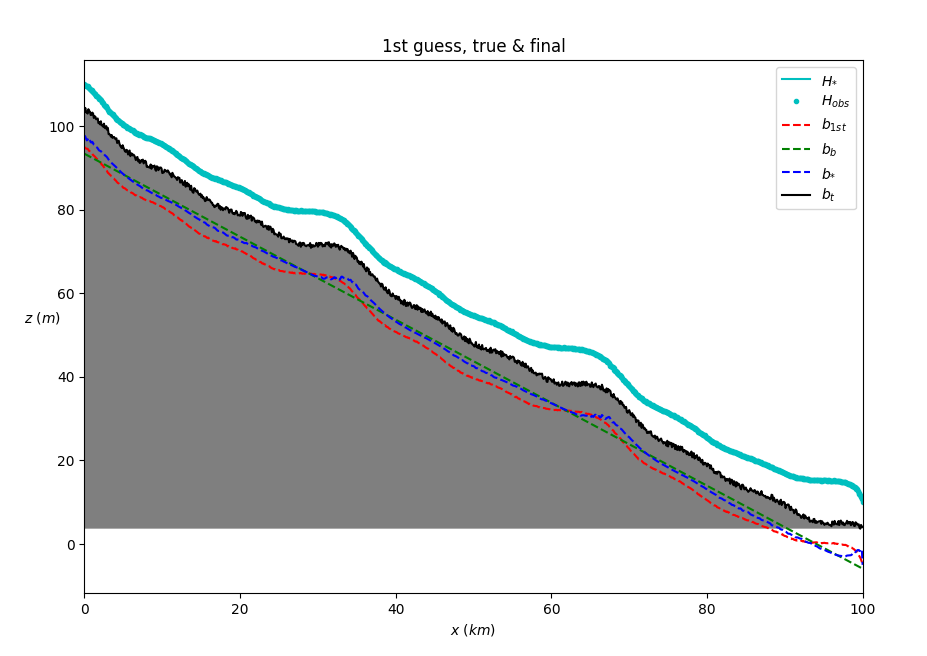
\includegraphics[width=\linewidth]{Images_Ayoub/With_Regularisation/Alpha_Const/Graphs/View.png}
        \caption{Vue du champ simulé avec \(\alpha=\tfrac18\).}
        \label{fig:wr-view}
    \end{minipage}
\end{figure}

L'analyse des résultats obtenus avec une régularisation de type background (\(\alpha_{\text{reg}} = \tfrac{1}{8}\)) permet de tirer plusieurs conclusions intéressantes :

\begin{itemize}
    \item La fonction de coût décroît de manière satisfaisante au cours des itérations. Cette décroissance est toutefois plus lente que dans le cas sans régularisation, ce qui est attendu puisque la régularisation introduit une contrainte supplémentaire à l’optimisation.
    
    \item Le choix de \(\alpha = \tfrac{1}{8}\), motivé par l'équilibrage des ordres de grandeur initiaux de \(J_{\text{obs}}\) et \(J_{\text{reg}}\), s'avère pertinent : les deux termes de coût sont de même ordre de grandeur tout au long de l’optimisation, ce qui permet un compromis équilibré entre fidélité aux données et proximité du background.
    
    \item La bathymétrie estimée \(b^\star\) est proche de la bathymétrie background \(b^b\), ce qui est typique d’un problème régularisé : la solution reste proche de l’état a priori tout en améliorant la cohérence avec les observations.
    
    \item La solution finale trouvée ne correspond pas exactement à la bathymétrie vraie \(b^{\text{true}}\), ce qui est tout à fait normal puisque l’algorithme utilise une bathymétrie background \(b^b\) qui en est relativement éloignée. La régularisation pousse naturellement la solution vers \(b^b\), tout en essayant de satisfaire les observations.
    
    
    \item On observe aussi que la norme du gradient décroit de manière régulière, bien qu’elle n’atteigne pas strictement zéro. Cela est tout à fait normal dans le cadre d’un problème contraint, où l’optimum ne correspond pas nécessairement à un gradient nul dans l’espace complet.
\end{itemize}


\subsubsection{Avec \(\alpha_{\text{reg}}\) décroissant}

La stratégie de régularisation décroissante consiste à imposer une forte contrainte en début d'optimisation pour stabiliser la solution autour du background, puis à réduire progressivement cette force pour permettre un ajustement plus précis aux observations. Cette approche hybride conduit à une convergence accélérée tout en maintenant une cohérence avec l’état a priori.

\begin{figure}[H]
    \centering
    % Première ligne : Coûts et Gradient
    \begin{minipage}[b]{0.48\linewidth}
        \centering
        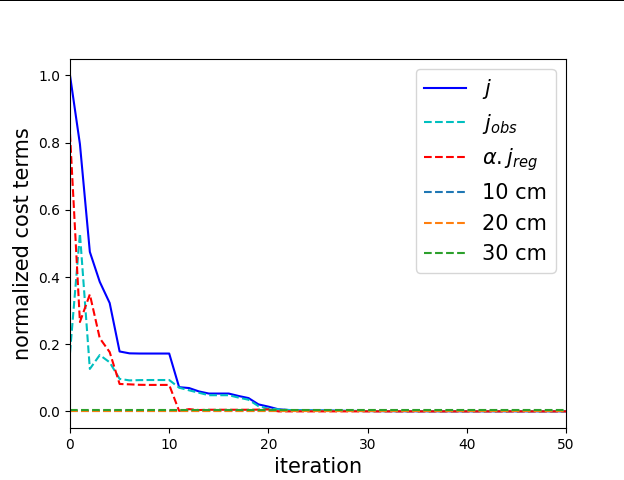
\includegraphics[width=\linewidth]{Images_Ayoub/With_Regularisation/Decreasing_Alpha/Costs.png}
        \caption{Évolution des coûts avec \(\alpha_{\text{reg}}\) décroissant.}
        \label{fig:dec-costs}
    \end{minipage}
    \hfill
    \begin{minipage}[b]{0.48\linewidth}
        \centering
        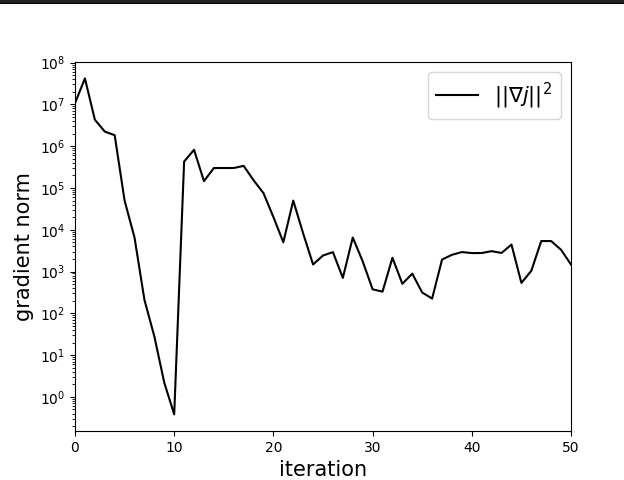
\includegraphics[width=\linewidth]{Images_Ayoub/With_Regularisation/Decreasing_Alpha/Gradient.png}
        \caption{Norme du gradient avec \(\alpha_{\text{reg}}\) décroissant.}
        \label{fig:dec-gradient}
    \end{minipage}
    
    \vspace{0.5cm}
    
    % Deuxième ligne : H et b
    \begin{minipage}[b]{0.48\linewidth}
        \centering
        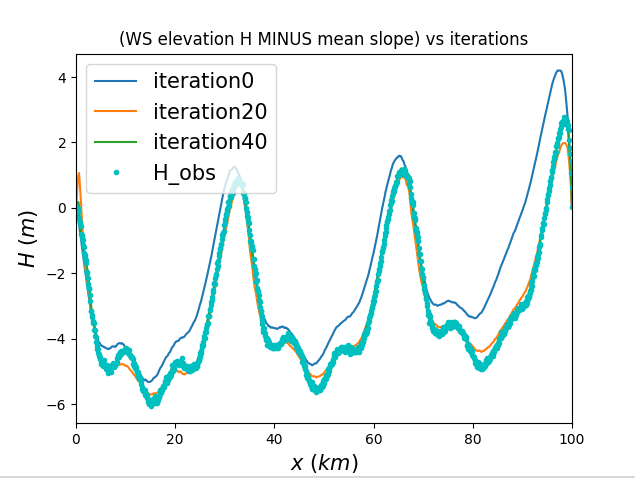
\includegraphics[width=\linewidth]{Images_Ayoub/With_Regularisation/Decreasing_Alpha/H_Comparaison.png}
        \caption{Comparaison du champ \(H\) estimé et des observations.}
        \label{fig:dec-h}
    \end{minipage}
    \hfill
    \begin{minipage}[b]{0.48\linewidth}
        \centering
        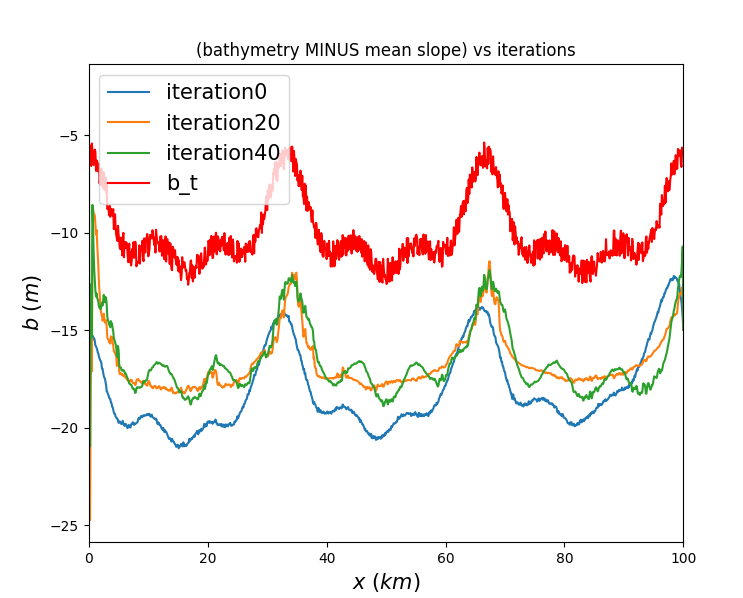
\includegraphics[width=\linewidth]{Images_Ayoub/With_Regularisation/Decreasing_Alpha/b_Comparaison.png}
        \caption{Comparaison de la bathymétrie estimée, du background et de la vérité.}
        \label{fig:dec-b}
    \end{minipage}
    
    \vspace{0.5cm}
    
    % Troisième ligne : Vue finale
    \begin{minipage}[b]{0.8\linewidth}
        \centering
        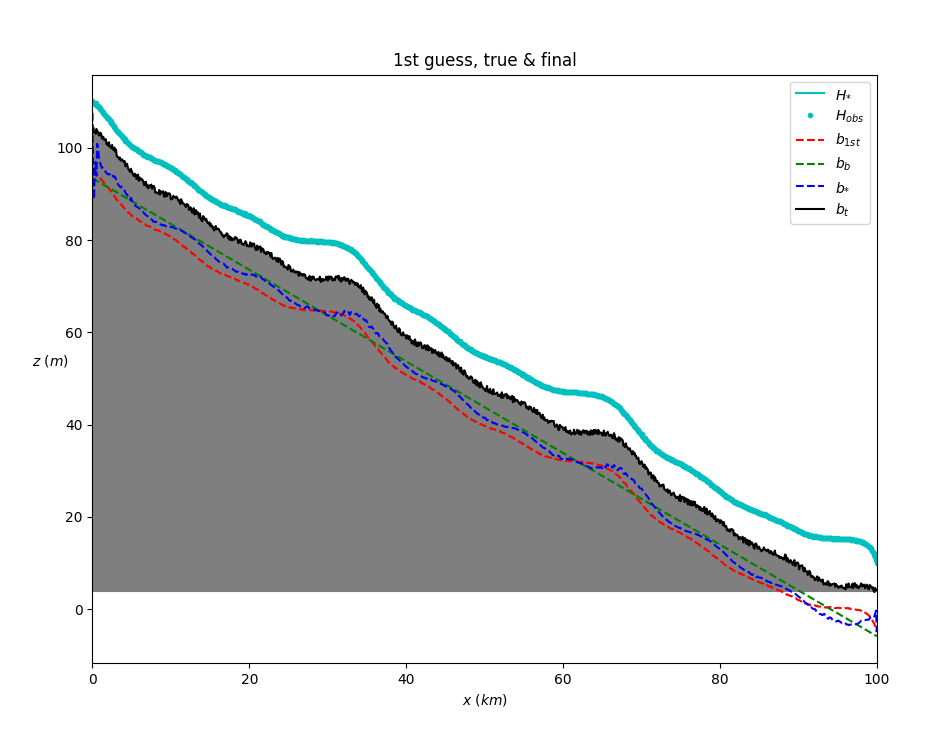
\includegraphics[width=\linewidth]{Images_Ayoub/With_Regularisation/Decreasing_Alpha/Viwe.png}
        \caption{Vue du champ simulé final avec \(\alpha_{\text{reg}}\) décroissant.}
        \label{fig:dec-view}
    \end{minipage}
\end{figure}



\paragraph{Analyse des résultats}
L'évolution de la loss (fonction de coût) montre qu'elle décroît plus rapidement avec une régularisation décroissante qu'avec un \(\alpha\) constant. On observe également des sauts dans la loss, causés par la diminution progressive de \(\alpha_{\text{reg}}\), qui modifie temporairement l'équilibre entre régularisation et ajustement aux observations. Cette méthode s'avère nettement plus efficace, permettant une convergence rapide et une meilleure adaptation aux données.

Cependant, malgré ces améliorations, l'estimation de la bathymétrie \(b\) ne parvient pas encore à atteindre la vérité \(b^{\text{true}}\), en raison de l'écart initial entre le \(b\) background et \(b^{\text{true}}\).



\subsection{Régularisation de type Gradient}

\begin{figure}[H]
    \centering
    % Première ligne : Coûts et Gradient
    \begin{minipage}[b]{0.48\linewidth}
        \centering
        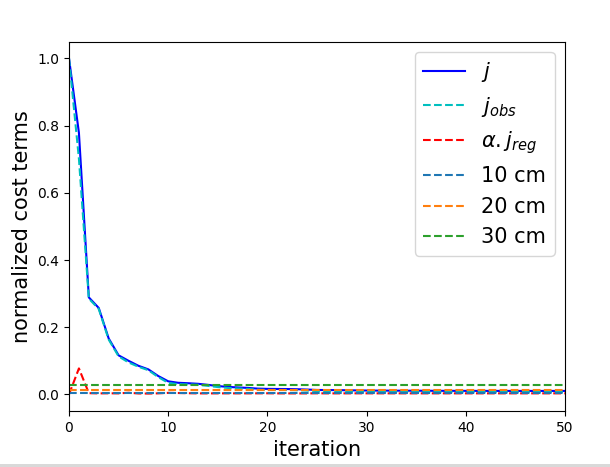
\includegraphics[width=\linewidth]{Images_Ayoub/With_Regularisation/Gradient/Costs.png}
        \caption{Évolution des coûts avec \(\alpha_{\text{reg}}\) décroissant.}
        \label{fig:dec-costs}
    \end{minipage}
    \hfill
    \begin{minipage}[b]{0.48\linewidth}
        \centering
        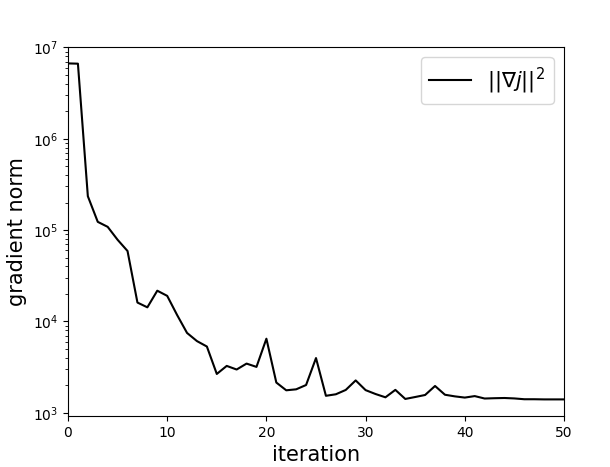
\includegraphics[width=\linewidth]{Images_Ayoub/With_Regularisation/Gradient/Gradient.png}
        \caption{Norme du gradient avec \(\alpha_{\text{reg}}\) décroissant.}
        \label{fig:dec-gradient}
    \end{minipage}
    
    \vspace{0.5cm}
    
    % Deuxième ligne : H et b
    \begin{minipage}[b]{0.48\linewidth}
        \centering
        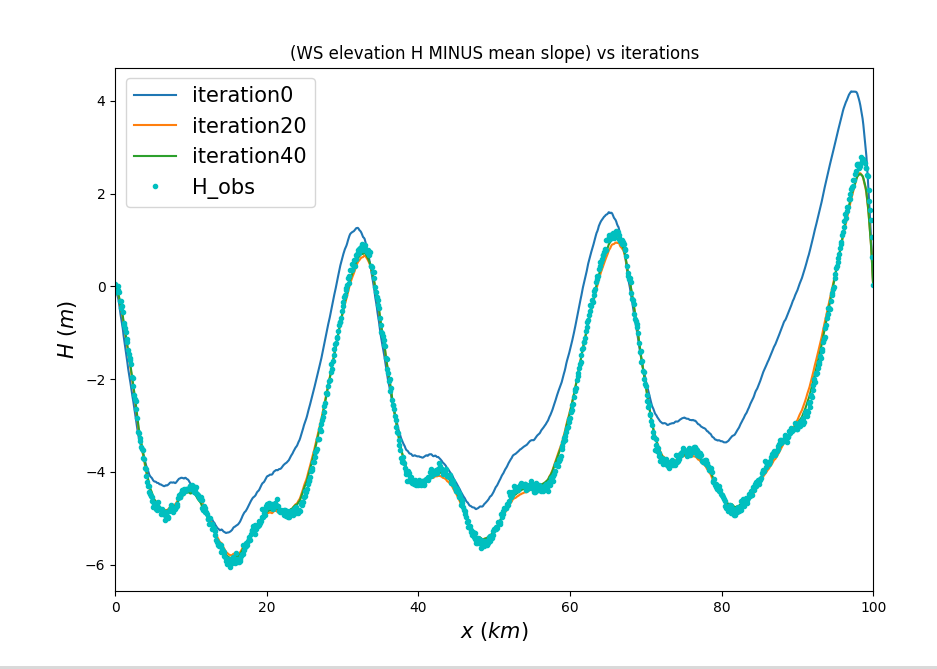
\includegraphics[width=\linewidth]{Images_Ayoub/With_Regularisation/Gradient/H_Comparaison.png}
        \caption{Comparaison du champ \(H\) estimé et des observations.}
        \label{fig:dec-h}
    \end{minipage}
    \hfill
    \begin{minipage}[b]{0.48\linewidth}
        \centering
        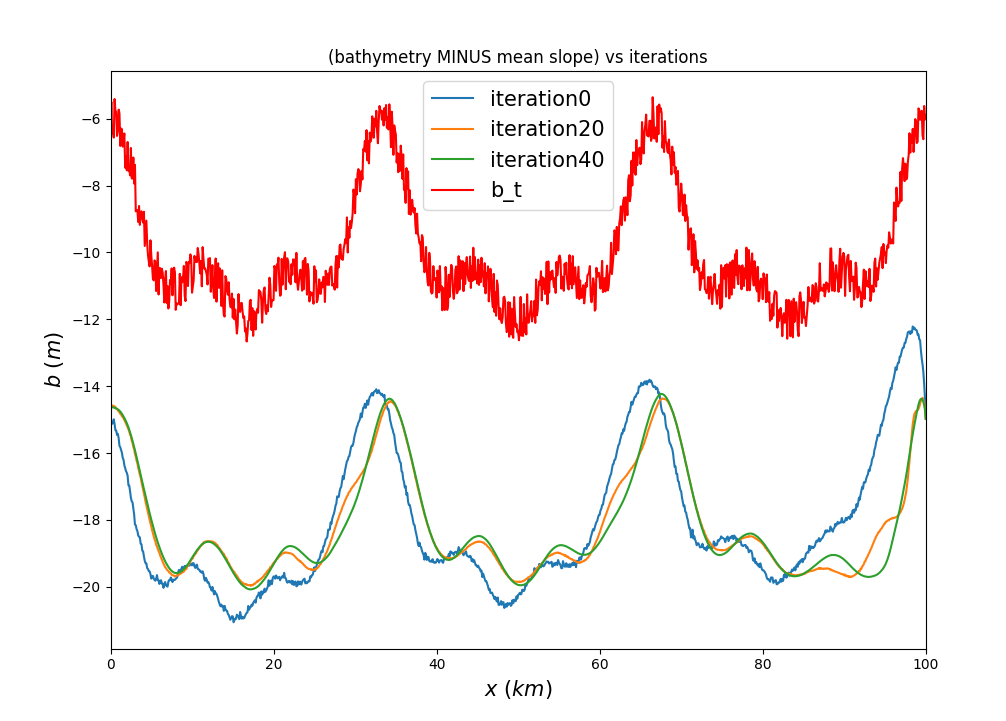
\includegraphics[width=\linewidth]{Images_Ayoub/With_Regularisation/Gradient/b_Comparaison.png}
        \caption{Comparaison de la bathymétrie estimée, du background et de la vérité.}
        \label{fig:dec-b}
    \end{minipage}
    
    \vspace{0.5cm}
    
    % Troisième ligne : Vue finale
    \begin{minipage}[b]{0.7\linewidth}
        \centering
        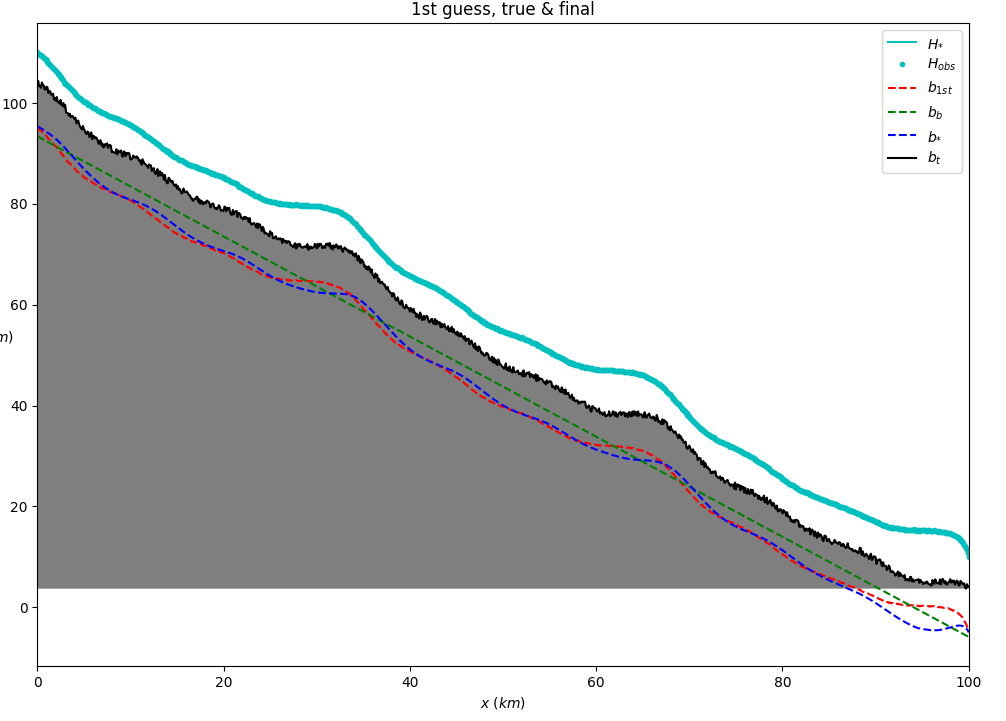
\includegraphics[width=\linewidth]{Images_Ayoub/With_Regularisation/Gradient/View.png}
        \caption{Vue du champ simulé final avec \(\alpha_{\text{reg}}\) décroissant.}
        \label{fig:dec-view}
    \end{minipage}
\end{figure}

\paragraph{Analyse des résultats}
L'évolution de la solution obtenue montre qu'elle est globalement lisse, ce qui traduit l'effet de la régularisation imposée. Les observations \( H_{\text{obs}} \) sont bien respectées, indiquant une bonne cohérence entre les données et le modèle estimé. Toutefois, malgré ces qualités, l'estimation de la bathymétrie \( b \) reste éloignée de la vérité \( b^{\text{true}} \), du à la nature mal posée du problème.


\section{Choix judicieux du \(b_{\text{background}}\) et du \(b_{\text{first}}\)}




Afin d'optimiser l'estimation, nous avons décidé de définir le \emph{prior depth} comme la moyenne de \(H_{\text{obs}} - b_{\text{true}}\). Cette approche offre une valeur représentative, contrairement à la méthode antérieure qui fixait le \emph{prior depth} à \(H_{\text{ref}}\) et calculait ensuite



\[
b_{\text{first}} = H_{\text{obs}} - 1.5 \times \text{prior depth},
\]



ce qui n'était pas toujours cohérent.

Ainsi maintenant, on va choisir :



\[
\text{prior\_depth} = \text{Mean}(H_{\text{obs}} - b_{\text{true}})
\]



Et poser ensuite :



\[
b_{\text{first}} = H_{\text{obs}} - 1 \times \text{prior\_depth}
\]











Par ailleurs, il est également envisageable de choisir la valeur à partir d'un seul point, ce qui est plus simple d'un point de vue opérationnel, bien que la moyenne sur l'ensemble des données reste préférable pour une meilleure représentativité. Nous avons aussi choisi de fixer \(b_{\text{background}}\) égal à \(b_{\text{first}}\). \newline

Pour améliorer la stabilité et obtenir des solutions plus lissées, nous avons opté pour une régularisation de type gradient dans laquelle la valeur de \(\alpha\) décroît, étant divisée par 10 à chaque 10 itération. Ce choix permet d'adapter progressivement l'influence du terme de régularisation au cours de l'optimisation.

Le tableau ci-dessous récapitule ces approches :

\begin{table}[H]
    \centering
    \begin{tabular}{|l|c|c|}
    \hline
                               & Méthode antérieure & Nouvelle approche \\ \hline
    Prior depth              & \(H_{\text{ref}}\) & \(\dfrac{1}{N}\displaystyle\sum_{i=1}^{N}\Bigl( H_{\text{obs},i} - b_{\text{true},i}\Bigr)\) \\ \hline
    \(b_{\text{first}}\)       & \(H_{\text{obs}} - 1.5 \times H_{\text{ref}}\) & \(H_{\text{obs}} - \text{prior depth}\) \\ \hline
    \(b_{\text{background}}\)  & --- & \(b_{\text{first}}\) \\ \hline
    Régularisation           & Constante & Gradient avec \(\alpha\) divisée par 10 à chaque 10 itérations \\ \hline
    \end{tabular}
    \caption{Comparaison des approches pour le choix du prior depth, \(b_{\text{first}}\), \(b_{\text{background}}\) et la régularisation.}
    \label{tab:prior_depth_bfirst}
\end{table}






\begin{figure}[H]
    \centering
    % Première ligne : Coûts et Gradient
    \begin{minipage}[b]{0.48\linewidth}
        \centering
        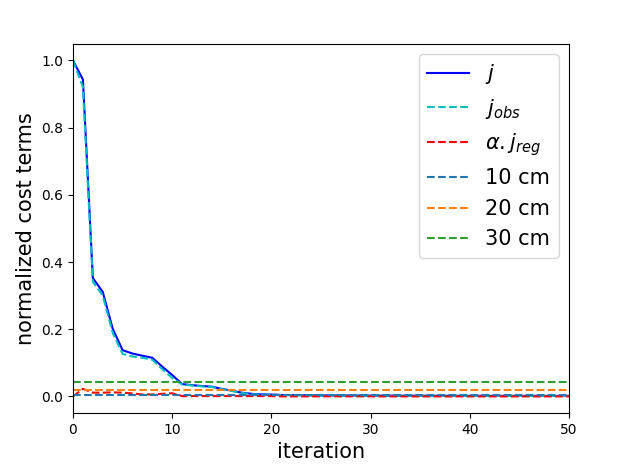
\includegraphics[width=\linewidth]{Images_Ayoub/h_connue/Costs.png}
        \caption{Évolution des coûts.}
        \label{fig:hconnue-costs}
    \end{minipage}
    \hfill
    \begin{minipage}[b]{0.48\linewidth}
        \centering
        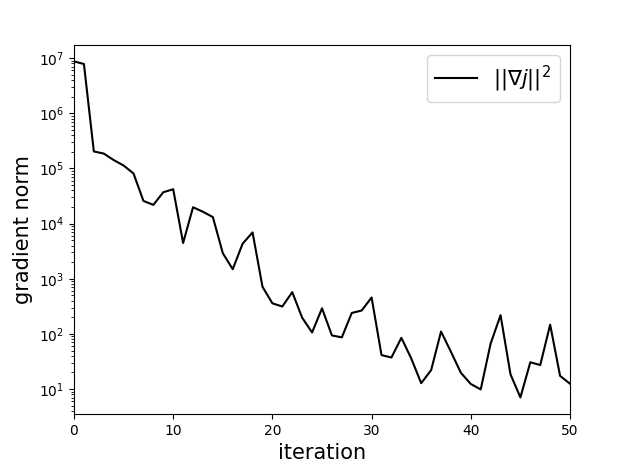
\includegraphics[width=\linewidth]{Images_Ayoub/h_connue/Gradient.png}
        \caption{Norme du gradient.}
        \label{fig:hconnue-gradient}
    \end{minipage}
    
    \vspace{0.5cm}
    
    % Deuxième ligne : Champ H et Bathymétrie
    \begin{minipage}[b]{0.48\linewidth}
        \centering
        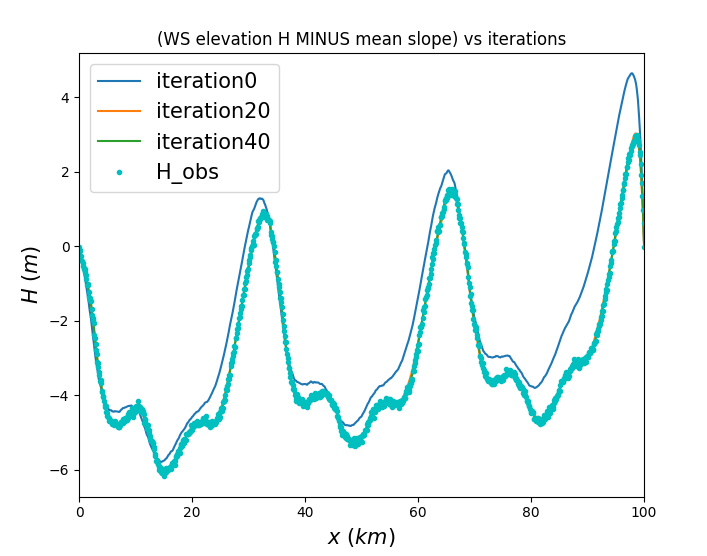
\includegraphics[width=\linewidth]{Images_Ayoub/h_connue/H_Comparaison.png}
        \caption{Comparaison du champ \(H\) estimé et des observations.}
        \label{fig:hconnue-Hcomparaison}
    \end{minipage}
    \hfill
    \begin{minipage}[b]{0.48\linewidth}
        \centering
        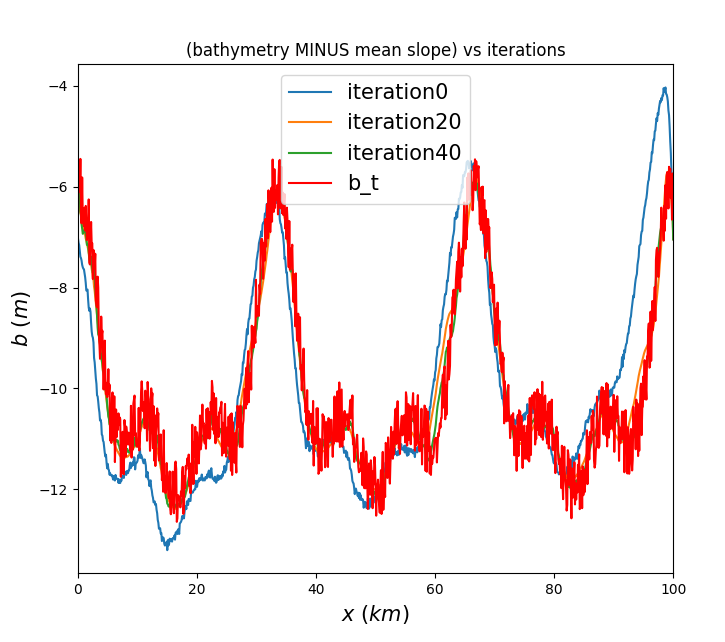
\includegraphics[width=\linewidth]{Images_Ayoub/h_connue/b_Comparaison.png}
        \caption{Comparaison de la bathymétrie estimée, du background et de la vérité.}
        \label{fig:hconnue-bcomparaison}
    \end{minipage}
    
    \vspace{0.5cm}
    
    % Troisième ligne : Vue finale
    \begin{minipage}[b]{0.8\linewidth}
        \centering
        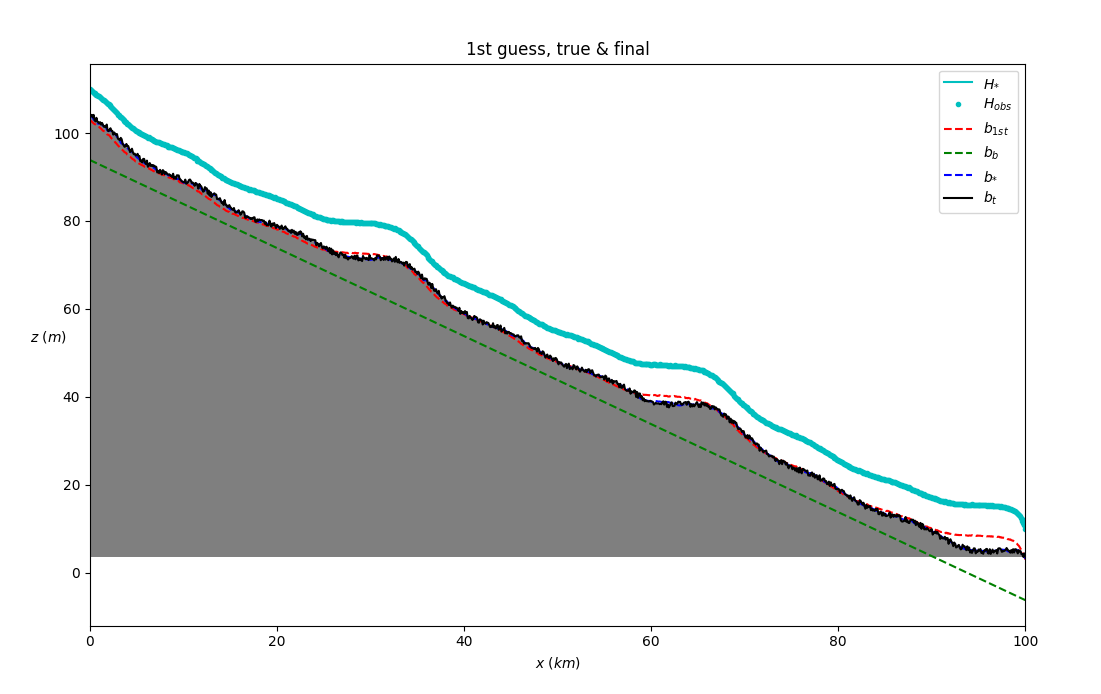
\includegraphics[width=\linewidth]{Images_Ayoub/h_connue/View.png}
        \caption{Vue du champ simulé final.}
        \label{fig:hconnue-view}
    \end{minipage}
\end{figure}




\paragraph{Analyse des résultats}
Tout d'abord, on remarque qu'en choisissant le \emph{prior depth} comme défini précédemment (la moyenne de \(H_{\text{obs}}-b_{\text{true}}\)), le \(b_{\text{first}}\) obtenu est sensiblement proche de \(b_{\text{true}}\). Cette proximité initiale permet d'améliorer significativement la convergence de l'algorithme, comme le montrent la diminution progressive de la loss et la stabilisation du gradient. 

De plus, nous avons expérimenté une approche alternative consistant à définir le \emph{prior depth} non pas comme la moyenne sur l'ensemble des données, mais simplement comme la différence à un point unique. Les résultats obtenus avec cette méthode montrent qu'elle fonctionne assez bien également, bien que le choix par moyenne reste préférable pour une robustesse accrue et une convergence plus homogène.

Ces observations confirment l'intérêt de notre choix méthodologique, qui permet d'obtenir des solutions initiales de \(b_{\text{first}}\) bien adaptées et favorise une meilleure convergence vers \(b_{\text{true}}\).




\section{Nos propres tests cases}

Dans cette étude, nous comparons deux méthodes d'initialisation du profil bathymétrique, \emph{b\_first}, en fonction de l'utilisation ou non d'une donnée a priori sur la profondeur. Pour chacune de ces méthodes, l'observation est réalisée avec une fréquence variant entre 3 et 30.



\subsection{Cas 1 : Absence d'information a priori (Unmonitored case)}

Lorsque aucune information complémentaire n'est utilisée, nous posons simplement :


\[
\text{prior\_depth} = h_{ref},
\]


ce qui revient à ne pas intégrer de correction basée sur une donnée a priori dans la construction de \emph{b\_first}. \newline 


La figure suivante permet de tracer les solution $b^*$ pour différentes valeurs initiales de $b_{first}$, et ceux pour les deux cas (fréquence 3 et fréquence 30). En plus, on a décidé de varier le type de régularisation (Type bb pour fréquence égale à 3) et (Type grad pour fréquence égale à $30$
)


\medskip
\begin{figure}[H]
    \centering
    \begin{subfigure}[b]{0.48\textwidth}
        \centering
        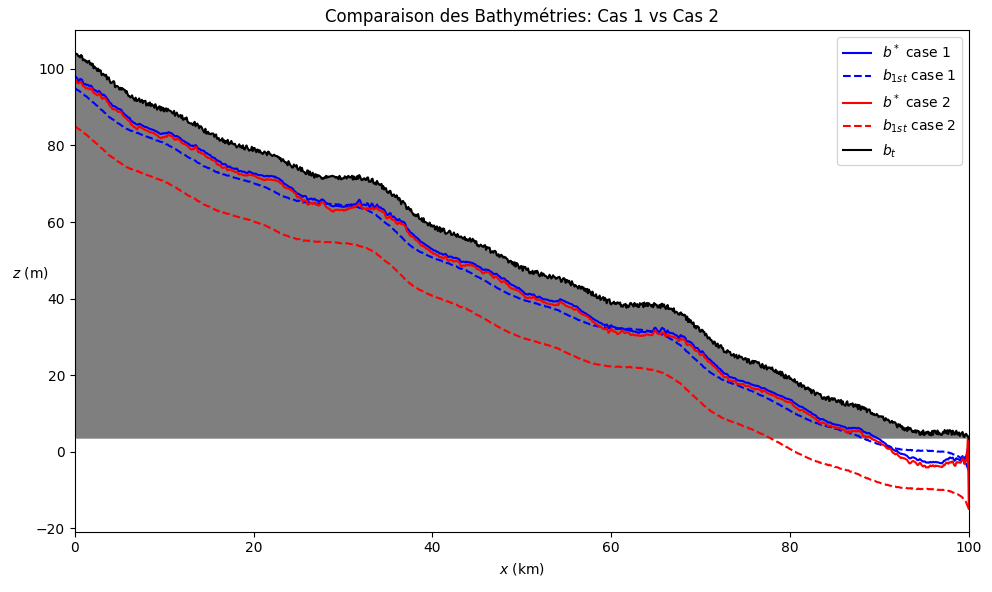
\includegraphics[width=\linewidth]{Images_Ayoub/Test_Cases_Tasks/Unmonitored/3/Pasted image.png}
        \caption{Fréquence 3 : Régularisation de type BB.}
        \label{fig:freq3_bb}
    \end{subfigure}
    \hfill
    \begin{subfigure}[b]{0.48\textwidth}
        \centering
        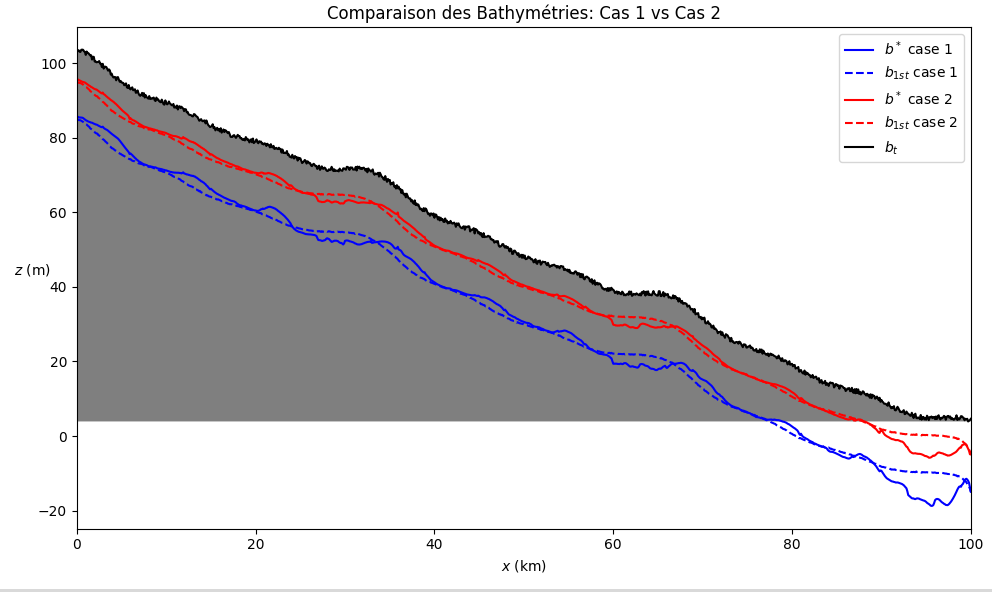
\includegraphics[width=\linewidth]{Images_Ayoub/Test_Cases_Tasks/Unmonitored/30/Pasted image.png}
        \caption{Fréquence 30 : Régularisation de type Grad.}
        \label{fig:freq30_grad}
    \end{subfigure}
    \caption{Solution pour l'estimation de la bathymétrie : pour une fréquence d'observation de 3, la régularisation utilisée est de type BB, tandis que pour une fréquence de 30, la régularisation de type Grad est appliquée.}
    \label{fig:comp_regul}
\end{figure}


\noindent\textbf{Analyse des résultats :}\

\begin{itemize}
    \item \textbf{Cas 1 (Fréquence 3 – régularisation BB) :}  
    Les solutions convergent vers une unique solution, confirmant l’unicité théorique du problème linéaire-quadratique. \newline

    \item \textbf{Cas 2 (Fréquence 30 – régularisation Grad) :}  
    Les solutions dépendent fortement du point de départ \( b_{1st} \) car l’unicité n’est plus garantie avec une régularisation d’ordre 1. Lorsque les observations sont rares, la non-unicité augmente et il devient nécessaire de disposer d’informations a priori plus précises.
\end{itemize}




\subsection{Cas 2 : L'utilisation d'une information a priori (Monitored case)}

Lorsqu'une valeur de profondeur a priori est disponible, celle-ci est obtenue à partir de l'observation au milieu du domaine :



\[
\text{prior\_depth} = h_{obs}\left(\frac{L}{2}\right) - b_{true}\left(\frac{L}{2}\right).
\]



Dans ce cas, le profil initial est défini par :



\[
b_{first} = h_{obs} - c \times \text{prior\_depth},
\]



où \( c \) représente une constante d'ajustement. Cette approche permet d'incorporer directement l'information a priori sur la profondeur pour ajuster le profil bathymétrique. De plus, des \textbf{contraintes d'égalité} sont imposées afin que le profil initial \( b_{start} \) soit strictement égale à \( b_{true} \) aux points d'observation, garantissant ainsi la cohérence entre la solution obtenue et les observations.

\begin{figure}[H]
    \centering
    \begin{subfigure}[b]{0.48\textwidth}
        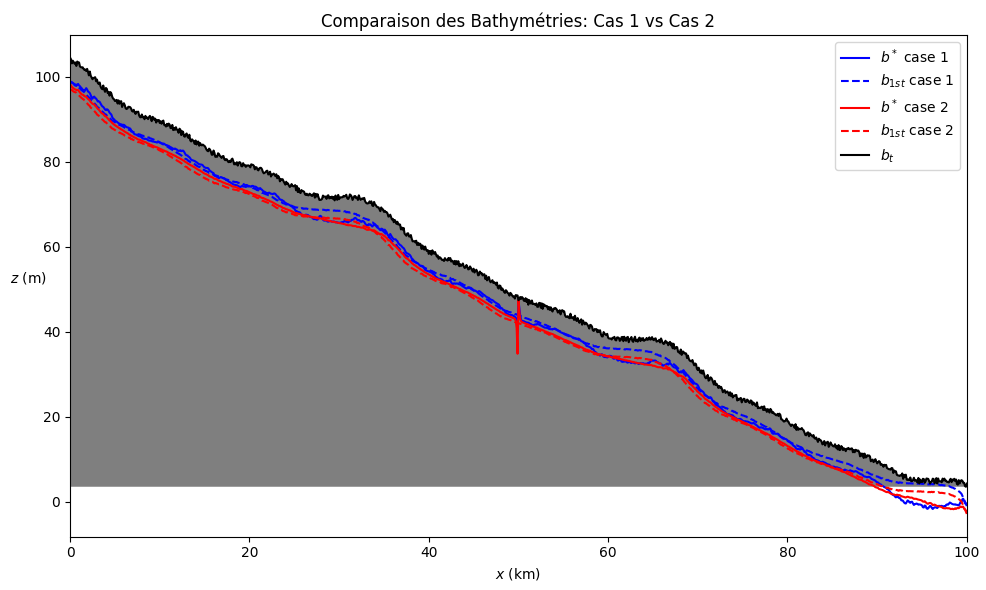
\includegraphics[width=\linewidth]{Images_Ayoub/Test_Cases_Tasks/Monitored/3/Pasted image.png}
        \caption{Cas 1 : Fréquence 3, régularisation de type BB.}
        \label{fig:cas1}
    \end{subfigure}
    \hfill
    \begin{subfigure}[b]{0.48\textwidth}
        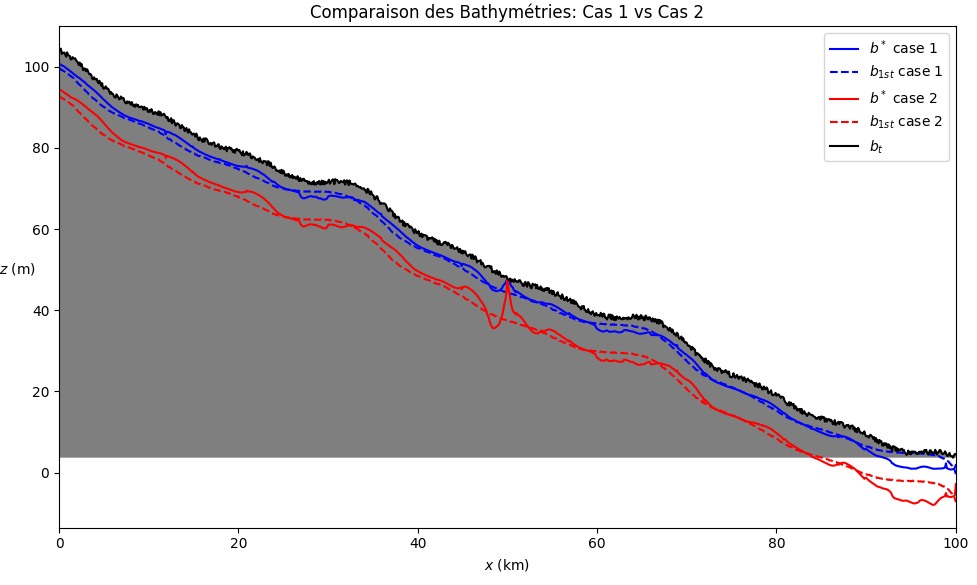
\includegraphics[width=\linewidth]{Images_Ayoub/Test_Cases_Tasks/Monitored/30/Pasted image.png}
        \caption{Cas 2 : Fréquence 30, régularisation de type Grad.}
        \label{fig:cas2}
    \end{subfigure}
    \caption{Comparaison des solutions pour deux fréquences d'observation : (a) avec une régularisation BB et (b) avec une régularisation Grad.}
    \label{fig:comparison}
\end{figure}

\noindent\textbf{Analyse des résultats :}\

\begin{itemize}
    \item \textbf{Cas 1 (Fréquence 3 – régularisation BB) :}  
    Les solutions convergent toujours presque vers une même solution, confirmant l’unicité théorique du problème linéaire-quadratiue. On remarque en plus qu'il y'a une petite perturbation dans la solution au point qui se trouve au milieu du domaine. Ceci est du à la contrainte d'égalité qu'on a imposé à la solution.

    \item \textbf{Cas 2 (Fréquence 30 – régularisation Grad) :}  
    Les solutions dépendent toujours fortement du point de départ \( b_{1st} \) car l’unicité n’est plus garantie avec une régularisation d’ordre 1. Toutefois, on remarque que la solution est beaucoup plus lisse que par rapport au cas numéro. Cela est du à la régularisation de type grad qu'on a imposé.
\end{itemize}




\section{Conclusion}

Cette étude a permis d'évaluer différentes approches d'estimation de bathymétrie par assimilation variationnelle de données (VDA). Les principaux résultats montrent que :

\begin{itemize}
    \item La \textbf{régularisation} est cruciale pour obtenir des solutions stables. La stratégie adaptative (coefficient $\alpha$ décroissant) s'est avérée particulièrement efficace, combinant rapidité de convergence et précision.

    \item Le choix des paramètres initiaux influence fortement les résultats :
    \begin{itemize}
        \item Une initialisation $b_{first} = H_{obs} - \text{prior\_depth}$ (moyenne des observations) donne de meilleurs résultats
        \item L'égalité $b_{background} = b_{first}$ améliore la cohérence de la solution
    \end{itemize}

    \item Deux cas ont été comparés :
    \begin{itemize}
        \item \textbf{Cas non monitoré} : Solution unique avec régularisation $L^2$ (problème quadratique convexe)
        \item \textbf{Cas monitoré} : Meilleure précision grâce aux contraintes d'égalité sur les points observés
    \end{itemize}

    \item Les limitations persistent pour :
    \begin{itemize}
        \item La reconstruction des hautes fréquences (effet de lissage du modèle direct)
        \item Les cas avec observations peu denses (nécessité d'informations a priori)
    \end{itemize}
\end{itemize}


\medskip

Ces résultats ouvrent la voie à plusieurs améliorations. L’introduction de contraintes physiques supplémentaires et l’exploration d’approches hybrides (e.g. VDA couplée à des modèles bayésiens ou de machine learning) pourraient améliorer la précision et la robustesse de nos modèles.




\end{document}
